\newcommand{\imprimircatalogacao}{%
	\noindent
	UNIVERSIDADE DO ESTADO DO RIO DE JANEIRO\\
	INSTITUTO POLITÉCNICO \\ 
    CURSO DE ENGENHARIA DE COMPUTAÇÃO\\
	
    \noindent
	Reitora: Gulnar Azevedo e Silva\\
    Vice-reitor: Bruno Rêgo Deusdará Rodrigues \\
	Diretor do Instituto Politécnico: Lucas Venâncio Pires de Carvalho Lima\\
	Coordenador de Curso: Rodrigo Lamblet Mafort\\
	
	\noindent
	Banca Avaliadora Composta por: \imprimirorientador~(Orientador)\\
	\hspace*{6.3cm}Prof. Dr. Nome do professor da banca\\
	\hspace*{6.3cm}Prof. Dr. Nome do professor da banca
	\\
    \\
	% \noindent
   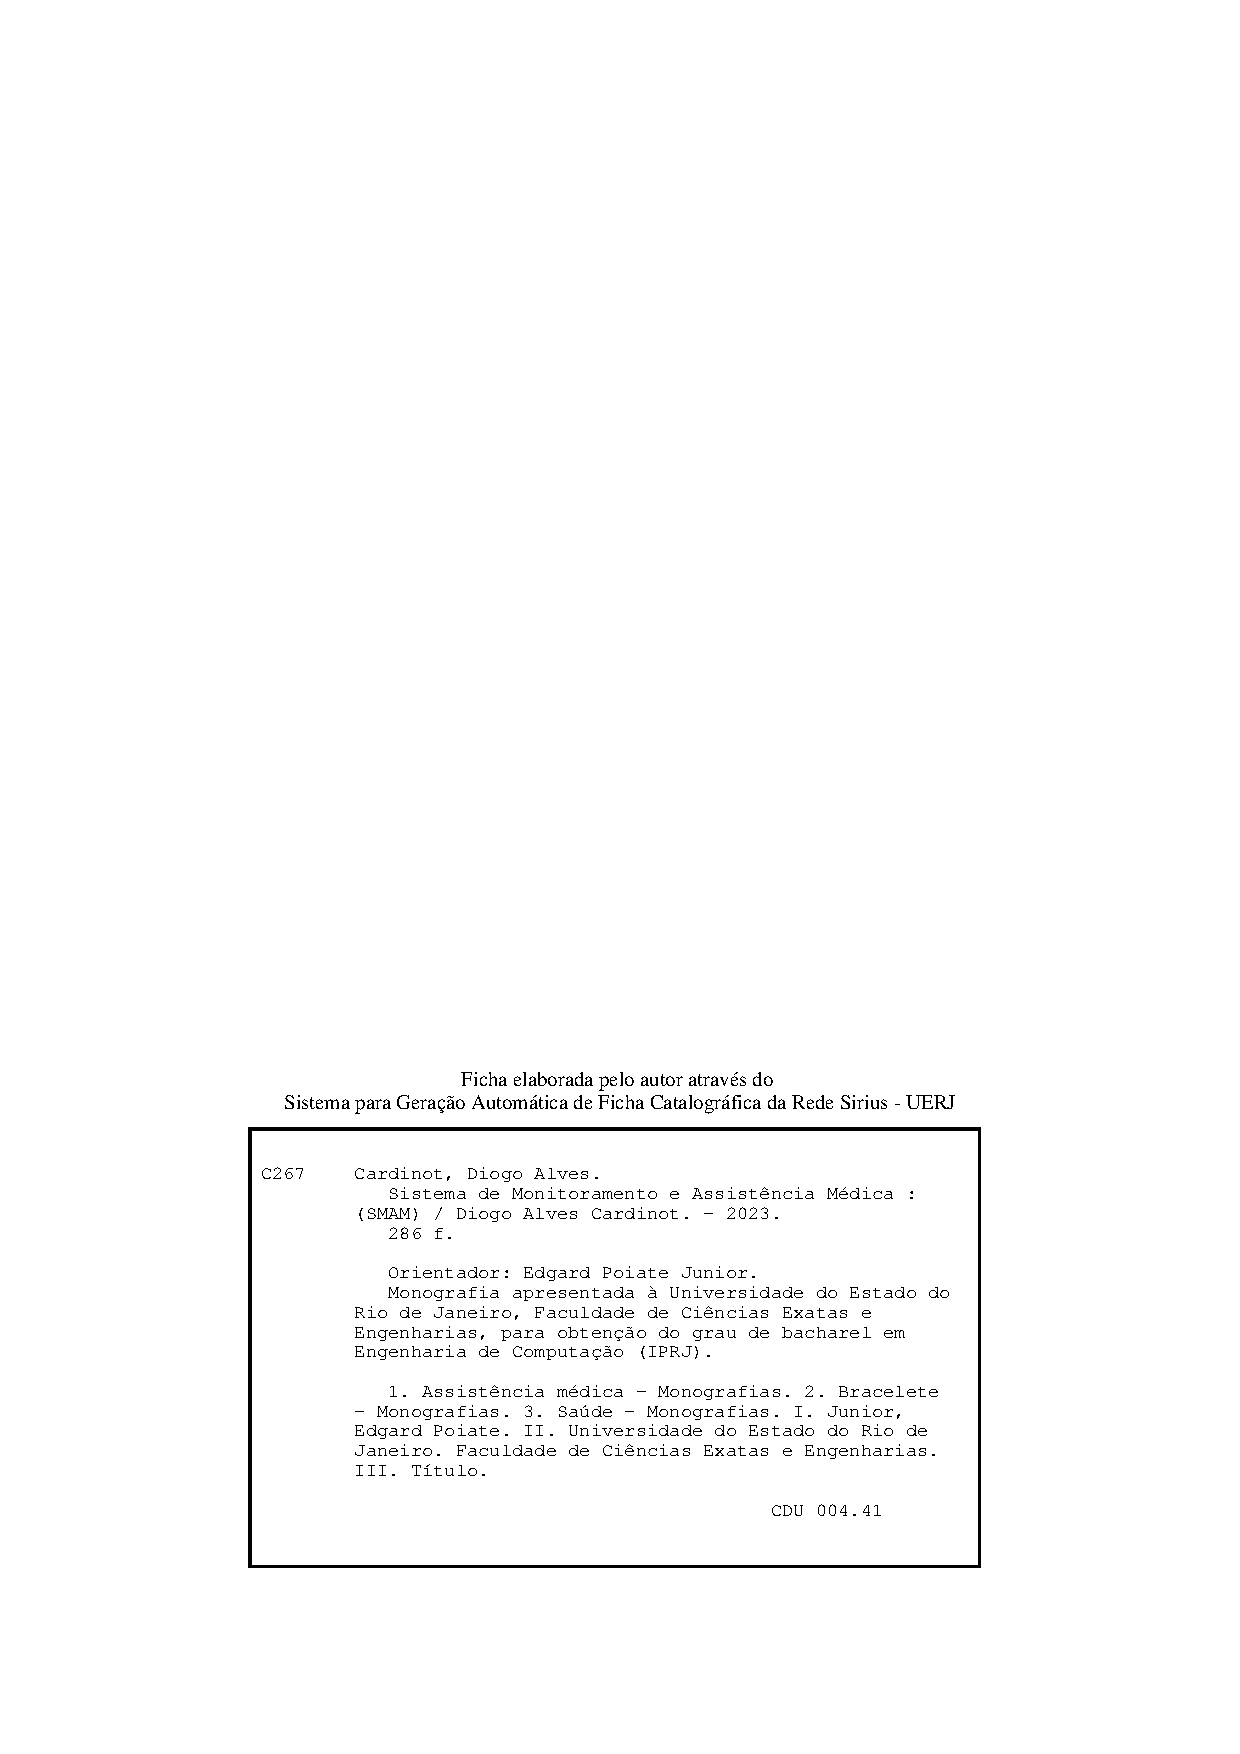
\includegraphics[
        page=1,
        trim={4cm 3cm 0cm 18cm},
	    clip,
	    width={17cm},
        height = {9cm}  %era 10
  ]{fichaBibli.pdf}
  %https://www.rsirius.uerj.br/servicos/elaboracao_ficha/instrucoes   gerar a sua
  %http://www.sirius.uerj.br/ficha/ficha104.php  preencher os dados

	%Endereço: UERJ - IPRJ,  Rua Bonfim, 25 - Prédio 5, Vila Amélia. CEP 28625-570 - Nova Friburgo - RJ - Brasil.\\
\noindent
Endereço: UERJ - IPRJ \\
\hspace*{2cm} CEP 28625-570 - Nova Friburgo - RJ - Brasil.\\

	\noindent
 Este trabalho nos termos da legislação que resguarda os direitos autorais é considerado de propriedade da Universidade do Estado do Rio de Janeiro (UERJ). É permitida a transcrição parcial de partes do trabalho, ou mencioná-lo, para comentários e citações, desde que sem propósitos comerciais e que seja feita a referência bibliográfica completa.
	\begin{flushright}
		\assinatura{\imprimirautor}
	\end{flushright}
}

\imprimircatalogacao